% Options for packages loaded elsewhere
\PassOptionsToPackage{unicode}{hyperref}
\PassOptionsToPackage{hyphens}{url}
\PassOptionsToPackage{dvipsnames,svgnames*,x11names*}{xcolor}
%
\documentclass[
  12pt,
  a4paper,
]{article}
\usepackage{lmodern}
\usepackage{setspace}
\usepackage{amsmath}
\usepackage{ifxetex,ifluatex}
\ifnum 0\ifxetex 1\fi\ifluatex 1\fi=0 % if pdftex
  \usepackage[T1]{fontenc}
  \usepackage[utf8]{inputenc}
  \usepackage{textcomp} % provide euro and other symbols
  \usepackage{amssymb}
\else % if luatex or xetex
  \usepackage{unicode-math}
  \defaultfontfeatures{Scale=MatchLowercase}
  \defaultfontfeatures[\rmfamily]{Ligatures=TeX,Scale=1}
  \setmainfont[]{Arial}
\fi
% Use upquote if available, for straight quotes in verbatim environments
\IfFileExists{upquote.sty}{\usepackage{upquote}}{}
\IfFileExists{microtype.sty}{% use microtype if available
  \usepackage[]{microtype}
  \UseMicrotypeSet[protrusion]{basicmath} % disable protrusion for tt fonts
}{}
\makeatletter
\@ifundefined{KOMAClassName}{% if non-KOMA class
  \IfFileExists{parskip.sty}{%
    \usepackage{parskip}
  }{% else
    \setlength{\parindent}{0pt}
    \setlength{\parskip}{6pt plus 2pt minus 1pt}}
}{% if KOMA class
  \KOMAoptions{parskip=half}}
\makeatother
\usepackage{xcolor}
\IfFileExists{xurl.sty}{\usepackage{xurl}}{} % add URL line breaks if available
\IfFileExists{bookmark.sty}{\usepackage{bookmark}}{\usepackage{hyperref}}
\hypersetup{
  pdftitle={Design Padrão para Output em PDF},
  colorlinks=true,
  linkcolor=RoyalBlue,
  filecolor=Maroon,
  citecolor=Blue,
  urlcolor=RoyalBlue,
  pdfcreator={LaTeX via pandoc}}
\urlstyle{same} % disable monospaced font for URLs
\usepackage[margin=.5in]{geometry}
\usepackage{color}
\usepackage{fancyvrb}
\newcommand{\VerbBar}{|}
\newcommand{\VERB}{\Verb[commandchars=\\\{\}]}
\DefineVerbatimEnvironment{Highlighting}{Verbatim}{commandchars=\\\{\}}
% Add ',fontsize=\small' for more characters per line
\usepackage{framed}
\definecolor{shadecolor}{RGB}{248,248,248}
\newenvironment{Shaded}{\begin{snugshade}}{\end{snugshade}}
\newcommand{\AlertTok}[1]{\textcolor[rgb]{0.94,0.16,0.16}{#1}}
\newcommand{\AnnotationTok}[1]{\textcolor[rgb]{0.56,0.35,0.01}{\textbf{\textit{#1}}}}
\newcommand{\AttributeTok}[1]{\textcolor[rgb]{0.77,0.63,0.00}{#1}}
\newcommand{\BaseNTok}[1]{\textcolor[rgb]{0.00,0.00,0.81}{#1}}
\newcommand{\BuiltInTok}[1]{#1}
\newcommand{\CharTok}[1]{\textcolor[rgb]{0.31,0.60,0.02}{#1}}
\newcommand{\CommentTok}[1]{\textcolor[rgb]{0.56,0.35,0.01}{\textit{#1}}}
\newcommand{\CommentVarTok}[1]{\textcolor[rgb]{0.56,0.35,0.01}{\textbf{\textit{#1}}}}
\newcommand{\ConstantTok}[1]{\textcolor[rgb]{0.00,0.00,0.00}{#1}}
\newcommand{\ControlFlowTok}[1]{\textcolor[rgb]{0.13,0.29,0.53}{\textbf{#1}}}
\newcommand{\DataTypeTok}[1]{\textcolor[rgb]{0.13,0.29,0.53}{#1}}
\newcommand{\DecValTok}[1]{\textcolor[rgb]{0.00,0.00,0.81}{#1}}
\newcommand{\DocumentationTok}[1]{\textcolor[rgb]{0.56,0.35,0.01}{\textbf{\textit{#1}}}}
\newcommand{\ErrorTok}[1]{\textcolor[rgb]{0.64,0.00,0.00}{\textbf{#1}}}
\newcommand{\ExtensionTok}[1]{#1}
\newcommand{\FloatTok}[1]{\textcolor[rgb]{0.00,0.00,0.81}{#1}}
\newcommand{\FunctionTok}[1]{\textcolor[rgb]{0.00,0.00,0.00}{#1}}
\newcommand{\ImportTok}[1]{#1}
\newcommand{\InformationTok}[1]{\textcolor[rgb]{0.56,0.35,0.01}{\textbf{\textit{#1}}}}
\newcommand{\KeywordTok}[1]{\textcolor[rgb]{0.13,0.29,0.53}{\textbf{#1}}}
\newcommand{\NormalTok}[1]{#1}
\newcommand{\OperatorTok}[1]{\textcolor[rgb]{0.81,0.36,0.00}{\textbf{#1}}}
\newcommand{\OtherTok}[1]{\textcolor[rgb]{0.56,0.35,0.01}{#1}}
\newcommand{\PreprocessorTok}[1]{\textcolor[rgb]{0.56,0.35,0.01}{\textit{#1}}}
\newcommand{\RegionMarkerTok}[1]{#1}
\newcommand{\SpecialCharTok}[1]{\textcolor[rgb]{0.00,0.00,0.00}{#1}}
\newcommand{\SpecialStringTok}[1]{\textcolor[rgb]{0.31,0.60,0.02}{#1}}
\newcommand{\StringTok}[1]{\textcolor[rgb]{0.31,0.60,0.02}{#1}}
\newcommand{\VariableTok}[1]{\textcolor[rgb]{0.00,0.00,0.00}{#1}}
\newcommand{\VerbatimStringTok}[1]{\textcolor[rgb]{0.31,0.60,0.02}{#1}}
\newcommand{\WarningTok}[1]{\textcolor[rgb]{0.56,0.35,0.01}{\textbf{\textit{#1}}}}
\usepackage{longtable,booktabs}
\usepackage{calc} % for calculating minipage widths
% Correct order of tables after \paragraph or \subparagraph
\usepackage{etoolbox}
\makeatletter
\patchcmd\longtable{\par}{\if@noskipsec\mbox{}\fi\par}{}{}
\makeatother
% Allow footnotes in longtable head/foot
\IfFileExists{footnotehyper.sty}{\usepackage{footnotehyper}}{\usepackage{footnote}}
\makesavenoteenv{longtable}
\usepackage{graphicx}
\makeatletter
\def\maxwidth{\ifdim\Gin@nat@width>\linewidth\linewidth\else\Gin@nat@width\fi}
\def\maxheight{\ifdim\Gin@nat@height>\textheight\textheight\else\Gin@nat@height\fi}
\makeatother
% Scale images if necessary, so that they will not overflow the page
% margins by default, and it is still possible to overwrite the defaults
% using explicit options in \includegraphics[width, height, ...]{}
\setkeys{Gin}{width=\maxwidth,height=\maxheight,keepaspectratio}
% Set default figure placement to htbp
\makeatletter
\def\fps@figure{htbp}
\makeatother
\setlength{\emergencystretch}{3em} % prevent overfull lines
\providecommand{\tightlist}{%
  \setlength{\itemsep}{0pt}\setlength{\parskip}{0pt}}
\setcounter{secnumdepth}{-\maxdimen} % remove section numbering
\pagestyle{plain}
\usepackage{lineno,sectsty,color,colortbl} % add

% Left justification of the text: see https://www.sharelatex.com/learn/Text_alignment
% \usepackage[document]{ragged2e} % already in the latex template
\newcommand{\bleft}{\begin{flushleft}}
\newcommand{\eleft}{\end{flushleft}}

\allsectionsfont{\mdseries\bfseries\color{RoyalBlue}}
\usepackage{booktabs}
\usepackage{longtable}
\usepackage{array}
\usepackage{multirow}
\usepackage{wrapfig}
\usepackage{float}
\usepackage{colortbl}
\usepackage{pdflscape}
\usepackage{tabu}
\usepackage{threeparttable}
\usepackage{threeparttablex}
\usepackage[normalem]{ulem}
\usepackage{makecell}
\usepackage{xcolor}
\ifluatex
  \usepackage{selnolig}  % disable illegal ligatures
\fi

\title{Design Padrão para Output em PDF}
\usepackage{etoolbox}
\makeatletter
\providecommand{\subtitle}[1]{% add subtitle to \maketitle
  \apptocmd{\@title}{\par {\large #1 \par}}{}{}
}
\makeatother
\subtitle{NA}
\author{}
\date{\vspace{-2.5em}}

\begin{document}
\maketitle

\setstretch{1.2}
\hypertarget{yaml-para-incluir-arquivo-.rmd}{%
\section{YAML para Incluir Arquivo .Rmd}\label{yaml-para-incluir-arquivo-.rmd}}

\begin{Shaded}
\begin{Highlighting}[]
\NormalTok{output}\SpecialCharTok{:}
\NormalTok{  bookdown}\SpecialCharTok{::}\NormalTok{pdf\_document2}\SpecialCharTok{:}
\NormalTok{    latex\_engine}\SpecialCharTok{:}\NormalTok{ xelatex}
\NormalTok{    fig\_caption}\SpecialCharTok{:}\NormalTok{ yes}
\NormalTok{    fig\_width}\SpecialCharTok{:} \FloatTok{3.5}
\NormalTok{    fig\_height}\SpecialCharTok{:} \FloatTok{2.0}
\NormalTok{    keep\_tex}\SpecialCharTok{:}\NormalTok{ yes}
\NormalTok{    number\_sections}\SpecialCharTok{:}\NormalTok{ no}
\NormalTok{    toc}\SpecialCharTok{:}\NormalTok{ no}
\NormalTok{    includes}\SpecialCharTok{:}
\NormalTok{      in\_header}\SpecialCharTok{:}\NormalTok{ header.tex}
      
\NormalTok{documentclass}\SpecialCharTok{:}\NormalTok{ article}
\NormalTok{papersize}\SpecialCharTok{:}\NormalTok{ a4}
\NormalTok{pagestyle}\SpecialCharTok{:}\NormalTok{ plain  }\CommentTok{\# plain, empty, headings}
\NormalTok{geometry}\SpecialCharTok{:}\NormalTok{ margin}\OtherTok{=}\NormalTok{.5in}
\NormalTok{linestretch}\SpecialCharTok{:} \FloatTok{1.2}
\NormalTok{mainfont}\SpecialCharTok{:}\NormalTok{ Arial}
\NormalTok{fontsize}\SpecialCharTok{:}\NormalTok{ 12pt}
\NormalTok{linkcolor}\SpecialCharTok{:}\NormalTok{ RoyalBlue}
\NormalTok{urlcolor}\SpecialCharTok{:}\NormalTok{ RoyalBlue}
\NormalTok{links}\SpecialCharTok{{-}}\NormalTok{as}\SpecialCharTok{{-}}\NormalTok{notes}\SpecialCharTok{:}\NormalTok{ false}
\end{Highlighting}
\end{Shaded}

\hypertarget{paruxe2metros-para-blocos-de-cuxf3digo}{%
\section{Parâmetros para Blocos de Código}\label{paruxe2metros-para-blocos-de-cuxf3digo}}

\begin{Shaded}
\begin{Highlighting}[]
\NormalTok{knitr}\SpecialCharTok{::}\NormalTok{opts\_chunk}\SpecialCharTok{$}\FunctionTok{set}\NormalTok{(}\AttributeTok{echo =}\NormalTok{ T,}
                      \AttributeTok{warning =}\NormalTok{ F,}
                      \AttributeTok{message =}\NormalTok{ F,}
                      \AttributeTok{fig.align =} \StringTok{"center"}\NormalTok{)}
\end{Highlighting}
\end{Shaded}

\hypertarget{paruxe2metros-para-formatauxe7uxe3o-de-gruxe1ficos}{%
\section{Parâmetros para Formatação de Gráficos}\label{paruxe2metros-para-formatauxe7uxe3o-de-gruxe1ficos}}

\begin{Shaded}
\begin{Highlighting}[]
\CommentTok{\# Função para padronizar o design dos gráficos}
\NormalTok{theme\_graph }\OtherTok{\textless{}{-}} \ControlFlowTok{function}\NormalTok{()\{}
  \FunctionTok{theme}\NormalTok{(}
    \AttributeTok{plot.title =} \FunctionTok{element\_text}\NormalTok{(}\AttributeTok{size =} \DecValTok{12}\NormalTok{),}
    \AttributeTok{plot.subtitle =} \FunctionTok{element\_text}\NormalTok{(}\AttributeTok{size =} \DecValTok{8}\NormalTok{),}
    \AttributeTok{plot.caption =} \FunctionTok{element\_text}\NormalTok{(}\AttributeTok{face =} \StringTok{"italic"}\NormalTok{, }\AttributeTok{size =} \DecValTok{7}\NormalTok{),}
    \AttributeTok{axis.title =} \FunctionTok{element\_text}\NormalTok{(}\AttributeTok{face =} \StringTok{"italic"}\NormalTok{, }\AttributeTok{size =} \DecValTok{7}\NormalTok{),}
    \AttributeTok{legend.position =} \StringTok{"bottom"}\NormalTok{,}
    \AttributeTok{legend.title =} \FunctionTok{element\_blank}\NormalTok{()}
\NormalTok{  )}
\NormalTok{\}}
\end{Highlighting}
\end{Shaded}

\hypertarget{pacotes-usados-no-artigo}{%
\section{Pacotes Usados no Artigo}\label{pacotes-usados-no-artigo}}

\begin{Shaded}
\begin{Highlighting}[]
\FunctionTok{library}\NormalTok{(tidyverse)}
\FunctionTok{library}\NormalTok{(gt)}
\FunctionTok{library}\NormalTok{(kableExtra)}
\end{Highlighting}
\end{Shaded}

\hypertarget{criauxe7uxe3o-e-formatauxe7uxe3o-de-tabelas}{%
\section{Criação e Formatação de Tabelas}\label{criauxe7uxe3o-e-formatauxe7uxe3o-de-tabelas}}

\begin{Shaded}
\begin{Highlighting}[]
\NormalTok{mtcars }\SpecialCharTok{\%\textgreater{}\%} 
  \FunctionTok{head}\NormalTok{() }\SpecialCharTok{\%\textgreater{}\%} 
\NormalTok{  kableExtra}\SpecialCharTok{::}\FunctionTok{kbl}\NormalTok{(}\AttributeTok{caption =} \StringTok{"Teste"}\NormalTok{,}
                  \AttributeTok{linesep =} \StringTok{"}\SpecialCharTok{\textbackslash{}\textbackslash{}}\StringTok{addlinespace"}\NormalTok{,}
                  \AttributeTok{booktabs =}\NormalTok{ T) }\SpecialCharTok{\%\textgreater{}\%} 
  \FunctionTok{kable\_styling}\NormalTok{(}\AttributeTok{position =} \StringTok{"center"}\NormalTok{,}
                \AttributeTok{font\_size =} \DecValTok{10}\NormalTok{,}
                \AttributeTok{full\_width =}\NormalTok{ F,}
                \AttributeTok{latex\_options =} \FunctionTok{c}\NormalTok{(}\StringTok{"HOLD\_position"}\NormalTok{,}\StringTok{"stripped"}\NormalTok{)) }\SpecialCharTok{\%\textgreater{}\%} 
\NormalTok{  kableExtra}\SpecialCharTok{::}\FunctionTok{row\_spec}\NormalTok{(}\AttributeTok{row =} \DecValTok{0}\NormalTok{, }
                       \AttributeTok{bold =}\NormalTok{ T,}
                       \AttributeTok{italic =}\NormalTok{ F,}
                       \AttributeTok{underline =}\NormalTok{ F,}
                       \AttributeTok{background =} \StringTok{"RoyalBlue"}\NormalTok{,}
                       \AttributeTok{color =} \StringTok{"white"}\NormalTok{)}
\end{Highlighting}
\end{Shaded}

\begin{table}[H]

\caption{\label{tab:unnamed-chunk-5}Teste}
\centering
\fontsize{10}{12}\selectfont
\begin{tabular}[t]{lrrrrrrrrrrr}
\toprule
\cellcolor{RoyalBlue}{\textcolor{white}{\textbf{ }}} & \cellcolor{RoyalBlue}{\textcolor{white}{\textbf{mpg}}} & \cellcolor{RoyalBlue}{\textcolor{white}{\textbf{cyl}}} & \cellcolor{RoyalBlue}{\textcolor{white}{\textbf{disp}}} & \cellcolor{RoyalBlue}{\textcolor{white}{\textbf{hp}}} & \cellcolor{RoyalBlue}{\textcolor{white}{\textbf{drat}}} & \cellcolor{RoyalBlue}{\textcolor{white}{\textbf{wt}}} & \cellcolor{RoyalBlue}{\textcolor{white}{\textbf{qsec}}} & \cellcolor{RoyalBlue}{\textcolor{white}{\textbf{vs}}} & \cellcolor{RoyalBlue}{\textcolor{white}{\textbf{am}}} & \cellcolor{RoyalBlue}{\textcolor{white}{\textbf{gear}}} & \cellcolor{RoyalBlue}{\textcolor{white}{\textbf{carb}}}\\
\midrule
Mazda RX4 & 21.0 & 6 & 160 & 110 & 3.90 & 2.620 & 16.46 & 0 & 1 & 4 & 4\\
\addlinespace
Mazda RX4 Wag & 21.0 & 6 & 160 & 110 & 3.90 & 2.875 & 17.02 & 0 & 1 & 4 & 4\\
\addlinespace
Datsun 710 & 22.8 & 4 & 108 & 93 & 3.85 & 2.320 & 18.61 & 1 & 1 & 4 & 1\\
\addlinespace
Hornet 4 Drive & 21.4 & 6 & 258 & 110 & 3.08 & 3.215 & 19.44 & 1 & 0 & 3 & 1\\
\addlinespace
Hornet Sportabout & 18.7 & 8 & 360 & 175 & 3.15 & 3.440 & 17.02 & 0 & 0 & 3 & 2\\
\addlinespace
Valiant & 18.1 & 6 & 225 & 105 & 2.76 & 3.460 & 20.22 & 1 & 0 & 3 & 1\\
\bottomrule
\end{tabular}
\end{table}

\hypertarget{criauxe7uxe3o-de-gruxe1ficos}{%
\section{Criação de Gráficos}\label{criauxe7uxe3o-de-gruxe1ficos}}

\begin{Shaded}
\begin{Highlighting}[]
\NormalTok{mtcars }\SpecialCharTok{\%\textgreater{}\%} 
\NormalTok{  ggplot2}\SpecialCharTok{::}\FunctionTok{ggplot}\NormalTok{()}\SpecialCharTok{+}
  \FunctionTok{geom\_point}\NormalTok{(}\AttributeTok{mapping =} \FunctionTok{aes}\NormalTok{(}\AttributeTok{x =}\NormalTok{ mpg, }\AttributeTok{y =}\NormalTok{ cyl))}\SpecialCharTok{+}
  \FunctionTok{theme\_graph}\NormalTok{()}
\end{Highlighting}
\end{Shaded}

\begin{center}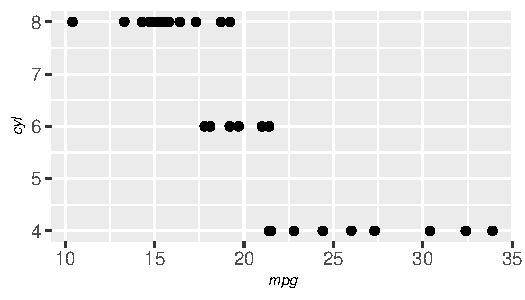
\includegraphics{standard_pagedown_template_files/figure-latex/unnamed-chunk-6-1} \end{center}

\end{document}
